
ASR and DEF, though produce similar visual indications (charcteristic map surface cracking), the mechanism of each is different. A short discussion of the two mechanisms is provided below.

\subsection{Alkali-Silica Reaction (ASR)}

Firstly identified by Stanton\cite{Stanton} over 70 years ago, ASR is a important reason of concrete deterioration. Since that time, ASR has been identified as a cause of deterioration of numerous concrete structures.

%Stanton, T. E. "Expansion of Concrete through Reaction between Cement and Aggregate." Publications of the American Society of Civil Engineers 66 (1940): 1781-1811.

Alkali silica reaction (ASR) is a deleterious chemical reaction, between some siliceous minerals in the aggregate and the alkalinity of the concrete.

As the result, a hydrophilic gel named ASR gel is formated and swells in the presence of moisture, causing the expansion of concrete. Figure \ref{ASR_mechanism} by Kreitman, K\cite{Kreitman} illustrates the mechanism of ASR.

%Kreitman, K. "Nondestructive Evaluation of Reinforced Concrete Structures Affected by Alkali-Silica Reaction and Delayed Ettringite Formation." MS Thesis, The University of Texas at Austin, Austin, Texas, 2011.

\begin{figure}[ht]
\centering
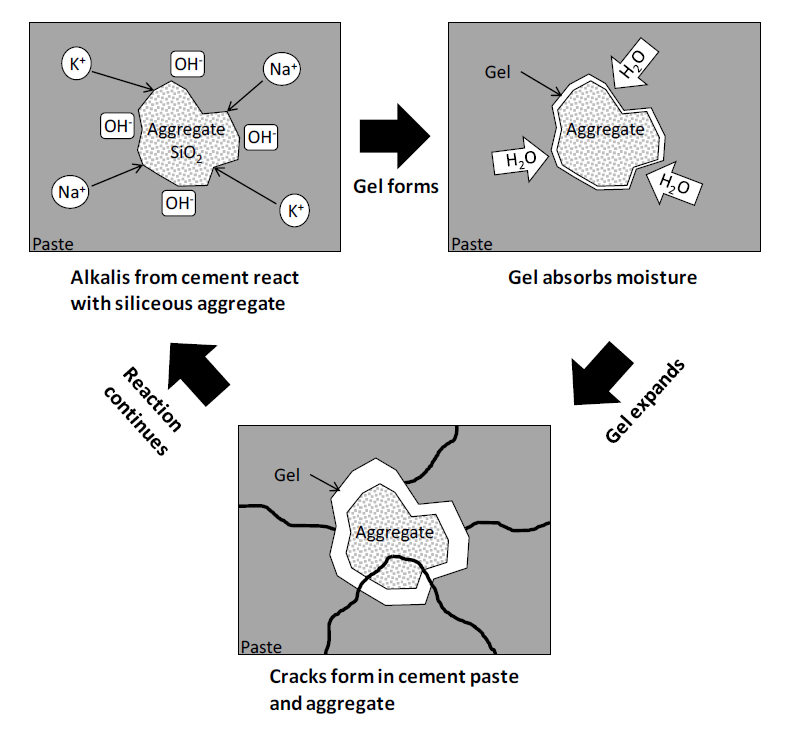
\includegraphics[width=.8\linewidth]{Reference/Kreitman.png}
  \caption{Mechanism of alkali-silica reaction [Kreitman 2011]}
  \label{ASR_mechanism}
\end{figure}

According to G.K. Glass\cite{Glass} in book Comprehensive Structural Integrity, 2003, factors which control the reaction rate and degree of expansion include the alkali content, the quantity of reactive aggregate and its particle size, the moisture content of the concrete and moisture content variations, temperature and the permeability of the concrete.

%G.K. Glass, in Comprehensive Structural Integrity, 2003

Although countermesures has yielded considerable success in minimize the risk of expansive ASR in new construction, the capability of ASR damaged concrete remains a major topic of ongoing research.

%%%%%%%%%%%%%%%%%%%%%%%%%%%%%%%%%%%%%%%%%%%%%%%%%%%%
\subsection{Delayed Ettringite Formation (DEF)}

Delayed Ettringite Formation (DEF) is a form of internal sulfate attack in concrete, driven by high curing temperatures and unfavorable cement chemistry (Kelham 1996\cite{Kelham}). Many laboratory studies have confirmed that 70$^\circ$C is the critical curing temperature for expansion due to DEF(H.F.W. Taylor et al., 2000\cite{Taylor}).

%Kelham, S. "The Effect of Cement Composition and Fineness on Expansion Associated with Delayed Ettringite Formation." Cement & Concrete Composites 18 (1996): 171-179.

%H.F.W Taylor, C. Famy, K.L. Scrivener. "Review: Delayed Ettringite Formation", Cement and Concrete Research 31(2001) 683-693

The hydration of cement and formation of C-S-H is greatly accelerated as curing temperature increases (Folliard, et al. 2006\cite{Folliard}). The rapidly growing “outer” C-S-H is different than that which forms at lower temperatures and traps dissolved sulfates before they can react to form ettringite, another normal product of cement hydration. With sustained temperatures above 70$^\circ$C, ettringite becomes thermodynamically unstable and either does not form or returns to solution.

%Folliard, K. J., et al. Preventing ASR/DEF In New Concrete: Final Report. Austin: Center for Transportation Research, 2006.

 Based on thermodynamics and X-ray diffraction observations, other hydration products, stable at high temperatures, such as calcium monosulfoaluminate (monosulfate) and hydrogarnet form instead from the decomposing ettringite and remaining aluminates, ferrites and sulfates in solution (Ramlochan 2003\cite{Ramlochan}).

 %Ramlochan, T. "The Effects of Pozzolans and Slag on the Expansion of Mortars and Concrete Cured at Elevated Temperature." PhD Thesis, Toronto: University of Toronto, 2003.

Once temperatures return to normal level, thermodynamics assist the formation of ettringite. Sulfates may be released from the C-S-H, then react with water and monosulfate, form ettringite, and lead to deleterious expansion and cracking of the concrete (Folliard et al, 2006\cite{Folliard}). A illustration of the mechanism of DEF is shown in Figure \ref{DEF_mechanism}.

 \begin{figure}[ht]
 \centering
 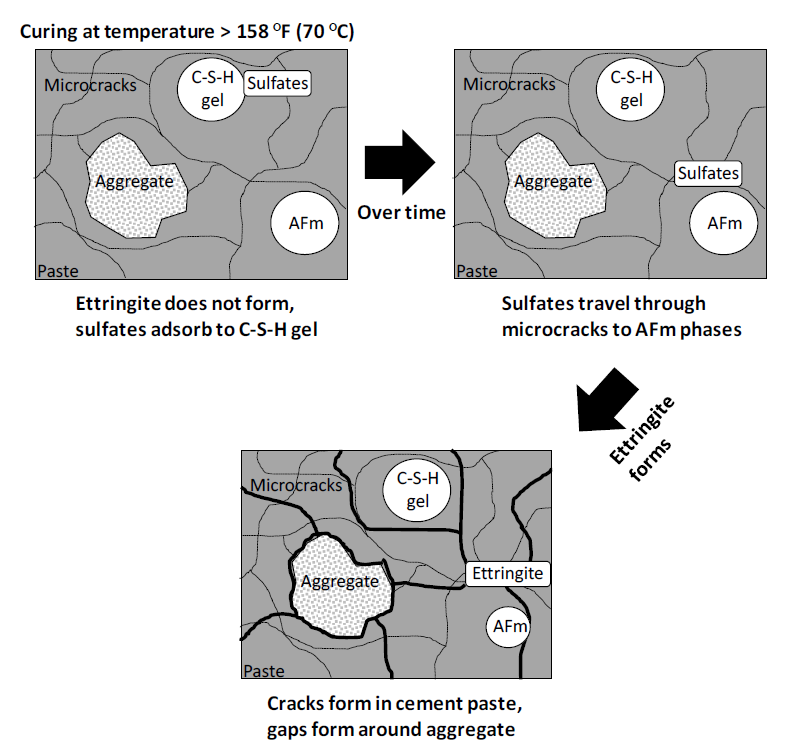
\includegraphics[width=.8\linewidth]{Reference/Kreitman2.png}
   \caption{Mechanism of delayed ettringite formation [Kreitman 2011]}
   \label{DEF_mechanism}
 \end{figure}
